% pdflatex -shell-escape software-analysis-main.tex
\documentclass[12pt,openany]{book}

\usepackage{kotex}
\usepackage{commath}
\usepackage{wasysym}
\usepackage{pifont} %http://ctan.org/pkg/pifont\usepackage{slantsc}
\usepackage{hyperref}
\usepackage{stmaryrd} %llbracket
\usepackage{adjustbox}
\usepackage{enumerate}

\usepackage{cite}
\usepackage[numbers]{natbib}
\usepackage{amsthm}

% Define custom theorem styles
\newtheoremstyle{dotless} % Name of the style
{3pt} % Space above
{3pt} % Space below
{\itshape} % Body font
{} % Indent amount
{\bfseries} % Theorem head font
{} % Punctuation after theorem head
{2.5mm} % Space after theorem head
{} % Theorem head spec

\newtheoremstyle{definitionstyle} % Name of the style
{3pt} % Space above
{3pt} % Space below
{} % Body font
{} % Indent amount
{\bfseries} % Theorem head font
{.} % Punctuation after theorem head
{2.5mm} % Space after theorem head
{} % Theorem head spec

% Applying custom styles
%\theoremstyle{dotless}
\newtheorem{theorem}{Theorem} % Theorem environment with section-wise numbering
\newtheorem*{theorem*}{Theorem} % Theorem environment with section-wise numbering
\newtheorem*{proposition*}{Proposition} % Theorem environment with section-wise numbering
\newtheorem*{corollary*}{Corollary} % Theorem environment with section-wise numbering
\newtheorem{proposition}[theorem]{Proposition} % Theorem environment with section-wise numbering
\newtheorem{lemma}[theorem]{Lemma} % Lemma shares the counter with theorem
\newtheorem{corollary}[theorem]{Corollary} % Corollary shares the counter with theorem

\theoremstyle{definitionstyle}
\newtheorem*{statement}{\textcolor{orange}{Statement}}
\newtheorem*{analysis}{\textcolor{magenta}{Analysis}}
\newtheorem*{pftactics}{\textcolor{teal}{Proof Tactics}}
\newtheorem*{observation}{\textcolor{Magenta}{Observation}}
\newtheorem{definition}{Definition} % Definition shares the counter with theorem
\newtheorem{example}{Example} % Example shares the counter with theorem
\newtheorem{exercise}{{Exercise}} % Example shares the counter with theorem
\newtheorem{remark}{Remark} % Remark shares the counter with theorem
\newtheorem*{note}{Note}

\newtheorem*{axiom*}{Axiom}
\newtheorem*{definition*}{Definition} % Definition shares the counter with theorem
\newtheorem*{example*}{Example} % Example shares the counter with theorem
\newtheorem*{exercise*}{\textcolor{violet}{Exercise}} % Example shares the counter with theorem
\newtheorem*{remark*}{Remark} % Remark shares the counter with theorem


% Colors
\usepackage[dvipsnames,table]{xcolor}
\definecolor{titleblue}{RGB}{0,53,128}
\definecolor{chaptergray}{RGB}{140,140,140}
\definecolor{sectiongray}{RGB}{180,180,180}

\definecolor{thmcolor}{RGB}{231, 76, 60}
\definecolor{defcolor}{RGB}{52, 152, 219}
\definecolor{lemcolor}{RGB}{155, 89, 182}
\definecolor{corcolor}{RGB}{46, 204, 113}
\definecolor{procolor}{RGB}{241, 196, 15}
\definecolor{execolor}{RGB}{90, 128, 127}

% Fonts
\usepackage[T1]{fontenc}
\usepackage[utf8]{inputenc}
\usepackage{newpxtext,newpxmath}
\usepackage{sectsty}
\allsectionsfont{\sffamily\color{titleblue}\mdseries}

% Page layout
\usepackage{geometry}
\geometry{a4paper,left=.8in,right=.6in,top=.75in,bottom=1in,heightrounded}
\usepackage{fancyhdr}
\fancyhf{}
\fancyhead[LE,RO]{\thepage}
\fancyhead[LO]{\nouppercase{\rightmark}}
\fancyhead[RE]{\nouppercase{\leftmark}}
\renewcommand{\headrulewidth}{0.5pt}
\renewcommand{\footrulewidth}{0pt}

% Chapter formatting
\usepackage{titlesec}
\titleformat{\chapter}[display]
{\normalfont\sffamily\Huge\bfseries\color{titleblue}}{\chaptertitlename\ \thechapter}{20pt}{\Huge}
\titleformat{\section}
{\normalfont\sffamily\Large\bfseries\color{titleblue!100!gray}}{\thesection}{1em}{}
\titleformat{\subsection}
{\normalfont\sffamily\large\bfseries\color{titleblue!75!gray}}{\thesubsection}{1em}{}

% Table of contents formatting
\usepackage{tocloft}
\renewcommand{\cftchapfont}{\sffamily\color{titleblue}\bfseries}
\renewcommand{\cftsecfont}{\sffamily\color{titleblue!100!gray}}
\renewcommand{\cftsubsecfont}{\sffamily\color{titleblue!75!gray}}
\renewcommand{\cftchapleader}{\cftdotfill{\cftdotsep}}

\usepackage{tcolorbox}
\tcbset{colback=white, arc=5pt}

\definecolor{defcolor}{RGB}{52, 152, 219}
\definecolor{procolor}{RGB}{241, 196, 15}
\definecolor{thmcolor}{RGB}{231, 76, 60}
\definecolor{lemcolor}{RGB}{155, 89, 182}
\definecolor{corcolor}{RGB}{46, 204, 113}
\definecolor{execolor}{RGB}{90, 128, 127}

% Define a new command for the custom tcolorbox
\newcommand{\defbox}[2][]{%
	\begin{tcolorbox}[colframe=defcolor, title={\color{white}\bfseries #1}]
		#2
	\end{tcolorbox}
}

\newcommand{\lembox}[2][]{%
	\begin{tcolorbox}[colframe=lemcolor, title={\color{white}\bfseries #1}]
		#2
	\end{tcolorbox}
}

\newcommand{\probox}[2][]{%
	\begin{tcolorbox}[colframe=procolor, title={\color{white}\bfseries #1}]
		#2
	\end{tcolorbox}
}

\newcommand{\thmbox}[2][]{%
	\begin{tcolorbox}[colframe=thmcolor, title={\color{white}\bfseries #1}]
		#2
	\end{tcolorbox}
}

\newcommand{\corbox}[2][]{%
	\begin{tcolorbox}[colframe=corcolor, title={\color{white}\bfseries #1}]
		#2
	\end{tcolorbox}
}
\usepackage{tikz}
\usepackage{tikz-cd}
\usepackage{tikz-3dplot}
\def\Circlearrowleft{\ensuremath{%
		\rotatebox[origin=c]{180}{$\circlearrowleft$}}}
\def\Circlearrowright{\ensuremath{%
		\rotatebox[origin=c]{180}{$\circlearrowright$}}}
\def\CircleArrowleft{\ensuremath{%
		\reflectbox{\rotatebox[origin=c]{180}{$\circlearrowleft$}}}}
\def\CircleArrowright{\ensuremath{%
		\reflectbox{\rotatebox[origin=c]{180}{$\circlearrowright$}}}}
\usetikzlibrary{
	3d, % For 3D drawing
	angles,
	arrows,
	arrows.meta,
	backgrounds,
	bending,
	calc,
	decorations.pathmorphing,
	decorations.pathreplacing,
	decorations.markings,
	fit,
	matrix,
	patterns,
	patterns.meta,
	positioning,
	quotes,
	shadows,
	shapes,
	shapes.geometric,
	trees
}

\usepackage{pgfplots}
\pgfplotsset{compat=newest} % Adjust to your version of pgfplots
\usepgfplotslibrary{statistics}
\usepackage[ruled,linesnumbered]{algorithm2e}
\usepackage{setspace}
\usepackage{algpseudocode}
\SetKwComment{Comment}{/* }{ */}
\SetKw{Break}{break}
\SetKw{Downto}{downto}
\SetKwProg{Fn}{Function}{:}{end}
\SetKwProg{Procedure}{procedure}{:}{end}
\SetKwProg{Construct}{Construct}{:}{end}
\SetKwFunction{KeyGen}{KeyGen}

%Listing
\usepackage{listings} %Code
\renewcommand{\lstlistingname}{Code}%
\definecolor{keyword}{RGB}{255, 0, 0}
\definecolor{identifier}{RGB}{0, 0, 255}
\definecolor{comment}{RGB}{0, 128, 0}
\definecolor{string}{RGB}{163, 21, 21}

\lstdefinestyle{c}{
	language=C,
	basicstyle=\ttfamily\small,
	keywordstyle=\color{keyword},
	identifierstyle=\color{identifier},
	commentstyle=\color{comment}\itshape,
	stringstyle=\color{string},
	showstringspaces=false,
	%	numberstyle=\tiny\color{gray},
	%	numbersep=5pt,
	frame=single,
	tabsize=4,
	captionpos=b,
	breaklines=true,
	breakatwhitespace=true,
	%	numbers=left
}
\newcommand{\A}{\mathbb{A}}
\newcommand{\B}{\mathbb{B}}
\newcommand{\C}{\mathbb{C}}
\newcommand{\F}{\mathbb{F}}
\newcommand{\N}{\mathbb{N}}
\newcommand{\Q}{\mathbb{Q}}
\newcommand{\R}{\mathbb{R}}
\newcommand{\Z}{\mathbb{Z}}

\newcommand{\cP}{\mathcal{P}}
\newcommand{\cR}{\mathcal{R}}

\newcommand{\pl}{\textsf{PL}\ }
\newcommand{\fol}{\textsf{FOL}\ }
\newcommand{\hol}{\textsf{HOL}\ }

\newcommand{\oracle}{\textsc{Oracle}}
\newcommand{\sub}[1]{\textsf{sub}\left(#1\right)}

\newcommand{\dom}{\mathsf{dom}}
\newcommand{\cdm}{\mathsf{cdm}}
\newcommand{\range}{\mathsf{range}}

\newcommand{\free}{\mathsf{free}}
\newcommand{\bound}{\mathsf{bound}}

\newcommand{\true}{\textcolor{red}{\texttt 1}}
\newcommand{\false}{\textcolor{red}{\texttt 0}}
\newcommand{\id}{\textnormal{id}}

\newcommand{\sol}{\textcolor{magenta}{\bf Sol}}
\newcommand{\ie}{i.\,e.}
\newcommand{\eg}{e.\,g.}
\newcommand{\wrt}{w.\,r.\,t.\ }
\newcommand{\aka}{a.\,k.\,a.\ }
\newcommand{\cf}{cf.\ }
\newcommand{\etc}{etc.\ }

\newcommand{\coa}{\mathsf{COA}}
\newcommand{\kpa}{\mathsf{KPA}}
\newcommand{\cpa}{\mathsf{CPA}}
\newcommand{\cca}{\mathsf{CCA}}
\newcommand{\acca}{\mathsf{CCA2}}\usetikzlibrary{arrows, positioning}

\begin{document}
	
	\begin{titlepage}
    \centering
    
    \vspace*{1cm}
    
    \Huge\textsf{\textbf{EasyCrypt - CodeCraftLab}}
    
    \vspace{0.5cm}
%   \LARGE\textsf{- A Deep Dive into Testing and Validation -}
    \LARGE\textsf{- Mastering the Art of EasyCrypt Programming -}
    
    \vspace{1.5cm}
    \textbf{Ji, Yong-Hyeon}

	\vspace{2cm}
%	\begin{figure}[h!]\centering
%	\begin{tikzpicture}
%		% Set colors for different logics
%		\definecolor{plcolor}{RGB}{255, 204, 204}
%		\definecolor{folcolor}{RGB}{204, 229, 255}
%		\definecolor{holcolor}{RGB}{204, 255, 204}
%		
%		% Draw the Higher-Order Logic (HOL) circle
%		\fill[holcolor] (0,0) circle (6cm);
%		\draw (0,0) circle (6cm);
%		\node at (0, 5.25) {\bf Higher-Order Logic (HOL)};
%		
%		% Draw the First-Order Logic (FOL) circle
%		\fill[folcolor] (0,0) circle (5cm);
%		\draw (0,0) circle (5cm);
%		\node at (0, 3.75) {\bf First-Order Logic (FOL)};
%		
%		% Draw the Propositional Logic (PL) circle
%		\fill[plcolor] (0,0) circle (3cm);
%		\draw (0,0) circle (3cm);
%		\node at (0, 0) {\bf Propositional Logic (PL)};
%		
%	\end{tikzpicture}
%	\end{figure}
%	\begin{center}
%	\adjustbox{scale=.9}{
%	\begin{tikzpicture}
%		
%		% Define colors
%		\definecolor{plcolor}{RGB}{255, 153, 153}
%		\definecolor{folcolor}{RGB}{153, 204, 255}
%		\definecolor{holcolor}{RGB}{153, 255, 153}
%		
%		% Draw the Higher-Order Logic (HOL) ellipse
%		\fill[holcolor, draw=black] (0,0) ellipse (8cm and 5cm);
%		\node at (0, 4.4) {\textbf{Higher-Order Logic (HOL)}};
%		
%		% Draw the First-Order Logic (FOL) ellipse
%		\fill[folcolor, draw=black] (0,0) ellipse (6cm and 4cm);
%		\node at (0, 3.4) {\textbf{First-Order Logic (FOL)}};
%		
%		% Draw the Propositional Logic (PL) ellipse
%		\fill[plcolor=, draw=black] (0,0) ellipse (4cm and 3cm);
%		\node at (0, 2.4) {\textbf{Propositional Logic (PL)}};
%		
%		% Add arrows to show inclusion
%%		\draw[thick,-Stealth] (0,0) -- (.5,-1.25) node[midway,above] {\footnotesize More expressive};
%%		\draw[thick,->] (2,1.2) -- (2.7,1.5);
%%		\draw[thick,->] (1.5,-1.2) -- (2.3,-1.5);
%		
%		% Add dimensions
%		\node at (1,-2.5) {\textbullet \, HOL: Functions, Predicates, Quantifiers};
%		\node at (.5,-1.25) {\textbullet \, FOL: Predicates, Quantifiers};
%		\node at (0,0) {\textbullet \, PL: Propositions};
%	\end{tikzpicture}}
%\end{center}
	
	\vspace{1.5cm}
    \vfill
    A document presented for the EasyCrypt
    
    \vspace{0.8cm}
    {\bf\large\textsf{Department of Information Security, Cryptology, and Mathematics}\par}
    {\large\textsf{College of Science and Technology}\par}
    {\large\textsf{Kookmin University}\par}
    \vspace{.25in}
    {\large \textsf{\today}\par}
    
%    \Large{Institution Name}\\
%    Date
\end{titlepage}


	\tableofcontents
	\newpage
	\section*{Symbols}
In this paper, symbols are defined as follows. \\ \ \\ 
$
\begin{array}{cl}
	I\models P & \text{$I$ satisfies $P$} \\
	I\not\models P & \text{$I$ does not satisfies $P$} \\
\end{array}
$
	
	\newpage
	\chapter{Mathematical Background}
	% Chapter 1. Installing EasyCrypt

\cite{StoughtonEasyCrypt}

The official EasyCrypt installation instructions are available on the EasyCrypt GitHub. Below is a summary of these instructions that also emphasizes the connection with the Emacs text editor. EasyCrypt can be run from the shell (command line) in batch mode, to check individual .ec files. But when proofs are constructed interactively this is done within Emacs, with the generic interface Proof General mediating between Emacs and EasyCrypt, which is running as a sub-process of Emacs.

These instructions are current for:
\begin{itemize}
	\item version 5.1.1 of the OCaml compiler;
	\item version 1.7.0 of \textsf{why3};
	\item version 2.5.2 of \textsf{alt-ergo}.
\end{itemize}

(EasyCrypt is implemented in OCaml, \textsf{why3} is the interface to SMT solvers used by EasyCrypt, and \textsf{alt-ergo} is one of SMT solvers you will need.) 

\section{Software Analysis}

\subsection{A Hard Limit}

\subsection{Trade-off}

\section{Basic Principle}
\subsection{Software Analysis based on Concrete Execution}
\subsection{Software Analysis based on Symbolic Execution}
\subsection{Software Analysis based on Abstract Execution}
	
	\newpage
	\chapter{Cryptographic Background}
	\section{Attacker Type}
\begin{itemize}
	\item $\coa$; Ciphertext-Only Attack
	\item $\kpa$; Known-Plaintext Attack
	\item $\cpa$; Chosen-Plaintext Attack
	\item $\cca$; Chosen-Ciphertext Attack
	\item $\acca$; Adaptive Chosen-Ciphertext Attack
\end{itemize}
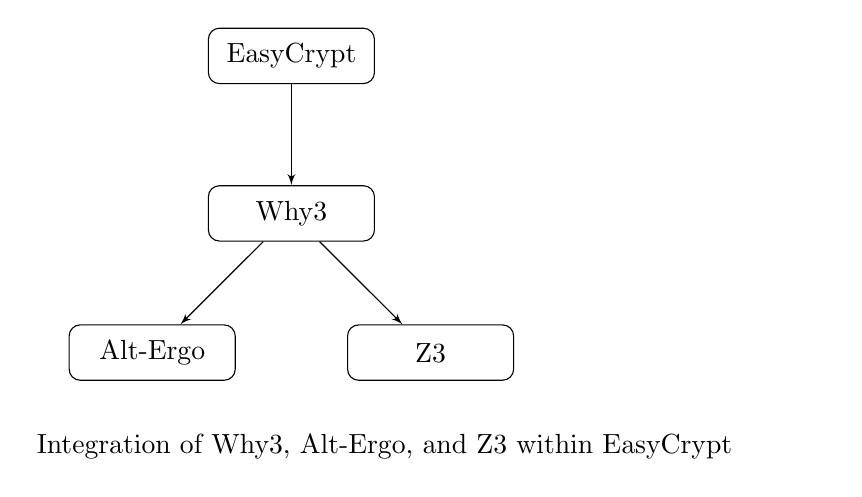
\begin{tikzpicture}[auto, node distance=2cm, >=latex']
	
	% Nodes
	\node [draw, rectangle, rounded corners, text centered, minimum height=2em, minimum width=6em] (easycrypt) {EasyCrypt};
	\node [draw, rectangle, rounded corners, below of=easycrypt, node distance=2cm, text centered, minimum height=2em, minimum width=6em] (why3) {Why3};
	\node [draw, rectangle, rounded corners, below left of=why3, node distance=2.5cm and 1.5cm, text centered, minimum height=2em, minimum width=6em] (altergo) {Alt-Ergo};
	\node [draw, rectangle, rounded corners, below right of=why3, node distance=2.5cm and 1.5cm, text centered, minimum height=2em, minimum width=6em] (z3) {Z3};
	
	% Arrows
	\draw [->] (easycrypt) -- (why3);
	\draw [->] (why3) -- (altergo);
	\draw [->] (why3) -- (z3);
	
	% Labels
	\node [below of=altergo, node distance=1.2cm] (label1) {};
	\node [below of=z3, node distance=1.2cm] (label2) {};
	\node [text width=10cm] at (label1 -| label2) {Integration of Why3, Alt-Ergo, and Z3 within EasyCrypt};
	
\end{tikzpicture}\\


\begin{itemize}
	\item $\mathcal{K}$: key space
	\item $\mathcal{N}$: nonce space
	\item $\mathcal{P}$: plaintext space
	\item $\mathcal{C}$: ciphertext space
\end{itemize}
\[
\texttt{used\_once}(n, \mathcal{N}) = n\in\mathcal{N}.
\]\[
\fullfunction{\texttt{used\_once}}{\mathcal{N}\times\set{\mathcal{N}}}{\set{0,1}}{(n,\mathcal{N})}{n\in\mathcal{N}}\]

\[
\texttt{used\_once}:\mathcal{N}\to[\set{\mathcal{N}}\to\set{0,1}]
\]
%현대 암호학에서는 공격자의 능력치에 따라 공격 유형을 다음과 같이 분류한다.
%1. 암호문 단독 공격()
%− 1개 이상의 암호문이 주어진 상황에서, 각 암호문에 대한 평문을 복원하는 공격
%2. 기지 평문 공격()
%− 동일한 키로 암호화한 평문/암호문 쌍이 1쌍 이상 주어진 상황에서, 동일한 키로 암호화한 새로운 암호문에 대한 평문을
%복원하는 공격
%3. 선택 평문 공격()
%− 공격자가 1개 이상의 원하는 평문에 대한 암호문을 얻은 후, 새롭게 주어진 암호문에 대한 평문을 복원하는 공격
%4. 선택 암호문 공격()12
%− 공격자가 1개 이상의 원하는 암호문에 대한 평문을 얻은 후, 새롭게 주어진 암호문에 대한 평문을 복원하는 공격

\newpage
\section{Initial Vectors}

\begin{itemize}
	\item $\mathcal{K}$: key space
	\item $\mathcal{N}$: nonce space
	\item $\mathcal{P}$: plaintext space
	\item $\mathcal{C}$: ciphertext space
\end{itemize}


\paragraph{Random IV}
Let $p\in\mathcal{P}$ and $k\in\mathcal{K}$. %The probability distribution of $E_k(p,IV)$ over the choice of $IV$ must approximate the uniform distribution over the $\mathcal{C}$, ensuring that:
\[
\Pr\left[E_k(p,IV)=c\right]\approx\frac{1}{\abs{\mathcal{C}}}\quad\text{for all}\ c\in\mathcal{C}.
\]

\paragraph{Nonce IV}
Let $p,q\in\mathcal{P}$ and $n,m\in\mathcal{N}$. \[
\Pr\left[E_k(p,n)=c=E_k(q,m)\right]=0\quad\text{if}\ p\neq q, n\neq m.
\]

\[
\lnot(a\lor b)\iff\lnot a \land \lnot b
\]

\begin{table}[h!]\centering\ttfamily\begin{tabular}{lc}
		split. & $\lnot(a\lor b)\Rightarrow \lnot a \land \lnot b$ \\
		move => not\_or. & $\lnot a \land\lnot b$ \\
		split. & $\lnot a$ \\
		case a. & $a\Rightarrow\lnot\top$ \\
		move => a\_true. & $\lnot\top$ \\
		$\vdots$ & $\vdots$
	\end{tabular}\end{table}
\begin{enumerate}
	\item $\lnot(a\lor b)\Rightarrow\lnot(a\land b)$
	\item $\lnot(a\lor b)\Rightarrow\lnot(a\land b)$
\end{enumerate}

	
	\newpage
	\chapter{Installing EasyCrypt}
	% Chapter 1. Installing EasyCrypt

\cite{StoughtonEasyCrypt}

The official EasyCrypt installation instructions are available on the EasyCrypt GitHub. Below is a summary of these instructions that also emphasizes the connection with the Emacs text editor. EasyCrypt can be run from the shell (command line) in batch mode, to check individual .ec files. But when proofs are constructed interactively this is done within Emacs, with the generic interface Proof General mediating between Emacs and EasyCrypt, which is running as a sub-process of Emacs.

These instructions are current for:
\begin{itemize}
	\item version 5.1.1 of the OCaml compiler;
	\item version 1.7.0 of \textsf{why3};
	\item version 2.5.2 of \textsf{alt-ergo}.
\end{itemize}

(EasyCrypt is implemented in OCaml, \textsf{why3} is the interface to SMT solvers used by EasyCrypt, and \textsf{alt-ergo} is one of SMT solvers you will need.) 

\section{Software Analysis}

\subsection{A Hard Limit}

\subsection{Trade-off}

\section{Basic Principle}
\subsection{Software Analysis based on Concrete Execution}
\subsection{Software Analysis based on Symbolic Execution}
\subsection{Software Analysis based on Abstract Execution}
		
	\newpage
	\appendix
	\chapter{Boolean Functions}
%	\input{appendix/sv-appendix-A}
	
	\bibliographystyle{plain}
	\bibliography{ec-references}	
\end{document}
